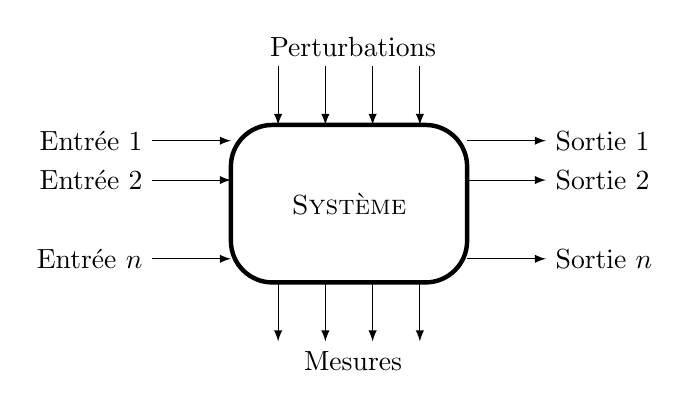
\begin{tikzpicture}
        \draw[-latex] (0.6,2.75) -- (0.6,2.0); 
        \draw[-latex] (1.2,2.75)node[above,xshift=1em] {Perturbations} -- (1.2,2.0); 
        \draw[-latex] (1.8,2.75) -- (1.8,2.0); 
        \draw[-latex] (2.4,2.75) -- (2.4,2.0); 
        \draw[ultra thick,rounded corners=15pt] (0,0) rectangle (3,2);
        \node (S) at (1.5,1) {\scshape Système};
        \draw[-latex] (-1,1.8) node[left] {Entrée 1} -- (0,1.8);
        \draw[-latex] (-1,1.3) node[left] {Entrée 2} -- (0,1.3);
        %\node[] at (-0.6,0.8) {\rotatebox{90}{\ldots}};
        \draw[-latex] (-1,0.3) node[left] {Entrée $n$} -- (0,0.3);
        \draw[-latex] (3,1.8) -- (4,1.8)node[right] {Sortie 1};
        \draw[-latex] (3,1.3) -- (4,1.3)node[right] {Sortie 2};
        %\node[] at (3.4,0.8) {\rotatebox{90}{\ldots}};
        \draw[-latex] (3,0.3) -- (4,0.3)node[right] {Sortie $n$};
        \draw[-latex] (0.6,0.0) -- (0.6,-0.75); 
        \draw[-latex] (1.2,0.0) -- (1.2,-0.75) node[below,xshift=1em] {Mesures}; 
        \draw[-latex] (1.8,0.0) -- (1.8,-0.75); 
        \draw[-latex] (2.4,0.0) -- (2.4,-0.75); 
\end{tikzpicture}
